\documentclass{beamer}
%\usetheme{Berlin}
%\usetheme{Ilmenau}
%\usetheme{Dresden}
%\usetheme{Berkeley}
%\usetheme{Bergen}
%\usetheme{Boadilla}
%\usetheme{Copenhagen}
%\usetheme{Hannover}
%\usetheme{Luebeck}
%\usetheme{AnnArbor}
%\usetheme{Darmstadt}
%\usetheme{Frankfurt}
\usetheme{Madrid}%azulito-li;la
%\usetheme{Warsaw}%int
%\usetheme{Antibes}
%\usetheme{CambridgeUS}%rojo-gris
%\usetheme{Malmoe}
%\usetheme{PaloAlto}

\usepackage{graphicx}
\usepackage[utf8]{inputenc}
\usepackage[spanish]{babel}
\usepackage{url}
%\usepackage{beamerthemeshadow}
\usepackage{caption}

\hyphenation{}


%Arreglos en el footnote
\makeatletter
\setbeamertemplate{footline}
{
  \leavevmode%
  \hbox{%
  \begin{beamercolorbox}[wd=.333333\paperwidth,ht=2.25ex,dp=1ex,center]{author in head/foot}%
    \usebeamerfont{author in head/foot}\insertshortauthor
  \end{beamercolorbox}%
  \begin{beamercolorbox}[wd=.58\paperwidth,ht=2.25ex,dp=1ex,center]{title in head/foot}%
    \usebeamerfont{title in head/foot}\inserttitle
  \end{beamercolorbox}%
  \begin{beamercolorbox}[wd=.1\paperwidth,ht=2.25ex,dp=1ex,center]{date in head/foot}%
    \usebeamerfont{date in head/foot}\insertframenumber{} / \inserttotalframenumber\hspace*{2ex} 
  \end{beamercolorbox}}%
  \vskip0pt%
}
\makeatother


\begin{document}
\title{Optimización de viajes compartidos en taxis utilizando algoritmos evolutivos}
\author[G. Fagúndez de los Reyes \and R. Massobrio]{Gabriel Fagúndez de los Reyes \and Renzo Massobrio} 
\institute[]{Facultad de Ingeniería,\\
Universidad de la República,\\
Montevideo, Uruguay}

\pgfdeclareimage[height=1.7cm]{university-logo}{logo}
\titlegraphic{\pgfuseimage{university-logo}}

%\date{\today} 
%\date{XII Simposio Argentino en Inteligencia Artificial}
\date{}

\frame{\frametitle{}\titlepage} 
\frame{\frametitle{Contenido}\tableofcontents} 

% ==============================================================
\section{Introducción}
\frame{\frametitle{Introducción} 
	\begin{block}{Acentuación ortográfica}
	La acentuación ortográfica en algunas palabras del idioma español elimina la ambigüedad de una oración.
	\end{block}

	\begin{block}{Clasificación de palabras con acento ortográfico}
	\begin{itemize}
		\item Sin ambigüedad: única forma correcta de escribir estas palabras, p.ej. \emph{acentuación}.
		\item Con ambigüedad: cambian su significado si son escritas con o sin acentuación ortográfica, p.ej.: verbos (\emph{canto/cantó, hable/hablé}), sustantivos (\emph{papa/papá, secretaria/secretaría}).
	\end{itemize}
	\end{block}
}

\frame{\frametitle{Introducción} 
	\begin{block}{Restauración de acentos ortográficos en palabras con ambigüedad}
		\begin{itemize}
			\item No es trivial.
			\item Involucra aspectos de desambiguación de significado. 
			\item Requiere examinar el contexto de cada palabra.
		\end{itemize}
	\end{block}
	
	\begin{block}{Adverbios interrogativos}
		\begin{itemize} 
			\item Gran dependencia con el contexto en el que aparecen.
			\item Particularmente difíciles de desambigüar.
		\end{itemize}
	\end{block}
	
	%En este trabajo se presenta la aplicación de dos técnicas de aprendizaje automático, CRF y SVM, para la resolución del problema de restauración automática de acentos ortográficos en adverbios interrogativos.
}

% ==============================================================
\section{Descripción del problema} 
\frame{\frametitle{Descripción del problema}
	\begin{block}{¿Qué es un adverbio interrogativo?}
		\begin{itemize} 
			\item Los adverbios son palabras invariables que complementan el significado de un verbo, un adjetivo u de otro adverbio. 
			\item Pueden funcionar de forma interrogativa, p.ej. \emph{¿dónde nació?}
			\item Pueden formularse de forma directa o indirecta, p.ej. \emph{¿Adónde os marcháis?} o \emph{Dime adónde saldréis}.
			\item En una frase pueden presentarse adverbios interrogativos y no interrogativos, p.ej. \emph{¿por \textbf{qué} algunas enfermedades de origen vírico, \textbf{como} los catarros o la gripe, pueden sufrirse en repetidas ocasiones?}
		\end{itemize}
	\end{block}
}

\frame{\frametitle{Descripción del problema}
	\begin{block}{Problema a resolver}
		Dado un texto del que fueron quitados todos los acentos ortográficos de sus adverbios, se debe clasificar cada palabra en una de las siguientes clases: 
		\begin{itemize}
			\item {\textbf{O}}. Toda palabra que no un adverbio.
			\item {\textbf{SIN\_TILDE}}. Si se trata de un adverbio no interrogativo.
			\item {\textbf{CON\_TILDE}}. Si se trata de un adverbio interrogativo.
		\end{itemize}
	\end{block}	
}

\frame{\frametitle{Descripción del problema}
	\begin{block}{Corpus de trabajo}
		\begin{itemize}
			\item Basado en la unión del corpus CESS Treebanks y CoNLL 2002.
			\item Consta de un total de aprox. $560.000$ tokens, de los cuales:
			\begin{itemize}
				\item $18.000$ son adverbios no interrogativos.
				\item $240$ son adverbios interrogativos.
			\end{itemize}
			\item Gran mayoría de los tokens del corpus no son adverbios.
			\begin{itemize}
				\item $99,96\%$ de \'exito en clasificador de línea base.
			\end{itemize}
		\end{itemize}
	\end{block}	
}

% ==============================================================
\section{Métodos para la resolución del problema}  
\frame{\frametitle{Métodos para la restauración de acentos}
	\begin{block}{Clasificadores propuestos}
		\begin{itemize}
			\item Se aborda el problema de la restauraci\'on de acentos ortogr\'aficos como un problema de clasificaci\'on.
			\item Según nuestro conocimiento no existen antecedentes de trabajos previos orientados a resolver el problema planteado.
			\item Se presentan dos técnicas de aprendizaje automático para la resolución del problema:
			\begin{itemize}
				\item Clasificador basado en Support Vector Machines (SVM).
				\item Clasificador basado en Conditional Random Fields (CRF).
			\end{itemize}
		\end{itemize}
	\end{block}
}

\frame{\frametitle{Clasificador basado en SVM}
		\begin{itemize}
			\item Implementado utilizando la herramienta SVM$^{light}$ y SVMTool.
			\begin{itemize}
				\item SVMTool es un generador de etiquetadores de secuencias.
			\end{itemize}
			\item Atributos utilizados para la clasificación.
			\begin{itemize}
				\item Ventana de 5 tokens centrada en el token a etiquetar.
				\item Etiquetas de los dos tokens previos al token a etiquetar.	
				\item Bigramas y trigramas de tokens y etiquetas de tokens.
				\begin{itemize}
					\item $(t_{-2},t_{-1})$, $(t_{0},t_{+1})$, $(e_{-2},e_{-1})$, $(t_{-1},t_{+1},t_{+2})$, etc.
				\end{itemize}
				\item Información de puntuación en la oración.
				\item Información tipográfica, p.ej.: mayúsculas, minúsculas, etc.
			\end{itemize}
		\end{itemize}
		\begin{figure}
			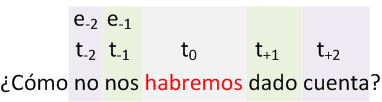
\includegraphics[scale=0.7]{ejemplos-svm} 
		\end{figure}
}

\frame{\frametitle{Clasificador basado en CRF}
		\begin{itemize}
				\item Implementado utilizando la herramienta MALLET.
			\item Atributos utilizados para la clasificación.
			\begin{itemize}
				\item Conjunciones de atributos del token anterior y siguiente.
				\begin{itemize}
					\item conj(-1,0) y conj(0,+1).
				\end{itemize}
				\item Atributo que marca la presencia de un token que generalmente precede o sucede a un adverbio.
				\begin{itemize}
					\item \texttt{\small PREV-SINT}, \texttt{\small NEXT-SINT}, \texttt{\small PREV-CONT} y \texttt{\small NEXT-CONT}.
				\end{itemize}
				\item Información de puntuación en la oración.
				\item Información tipográfica, p.ej. mayúsculas, minúsculas, etc.
			\end{itemize}
		\end{itemize}
		\begin{figure}
			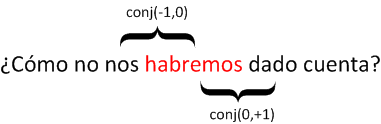
\includegraphics[scale=0.7]{ejemplos-crf} 
		\end{figure}
}

% ==============================================================
\section{Evaluación}
\begin{frame}
	\frametitle{Evaluación}
	\begin{block}{Metodología de evaluación}
		\begin{itemize}
			\item Se dividió el corpus en $10$ partes de tamaño similar.
			\item Se realizaron 10 entrenamientos con $\frac{9}{10}$ del corpus y se evaluó utilizando el $\frac{1}{10}$ restante.
			\item Se utilizaron métricas clásicas para la evaluación.
			\begin{itemize}
				\item Precisión, Recall y Medida-F.
			\end{itemize}
		\end{itemize}
	\end{block}
\end{frame}

\frame{\frametitle{Evaluación}
	\begin{center}
		\captionof{table}{Matriz de confusión del clasificador basado en SVM.}
		\small
		\begin{tabular}{|r||r|r|r|}
			\hline
				& \multicolumn{1}{c|}{\textbf{~O~}}
				& \multicolumn{1}{c|}{\textbf{SIN\_TILDE}}
				& \multicolumn{1}{c|}{\textbf{CON\_TILDE}} \\
			\hline\hline
			\textbf{O} & 54322,1 & 0,0 & 0,0 \\ \hline
			\textbf{SIN\_TILDE} & 0,0 & 1867,4 & 0,3 \\ \hline
			\textbf{CON\_TILDE} & 0,0 & 19,3 & 4,5 \\ 
			\hline
		\end{tabular}
	\end{center}
	\begin{center}
		\captionof{table}{Matriz de confusión del clasificador basado en CRF.}
		\small
		\begin{tabular}{|r||r|r|r|}
			\hline
				& \multicolumn{1}{c|}{\textbf{~O~}}
				& \multicolumn{1}{c|}{\textbf{SIN\_TILDE}}
				& \multicolumn{1}{c|}{\textbf{CON\_TILDE}} \\
			\hline\hline
			\textbf{O} & 54322,1 & 0,0 & 0,0 \\ \hline
			\textbf{SIN\_TILDE} & 0,0 & 1867,7 & 0,8 \\ \hline
			\textbf{CON\_TILDE} & 0,1 & 16,0 & 7,7 \\ 
			\hline
		\end{tabular}
	\end{center}
}

\begin{frame}
	\frametitle{Evaluación}
	\begin{block}{Análisis experimental}
		\begin{itemize}
			\item Confusión en la clasificasión de adverbios interrogativos.
			\begin{itemize}
				\item $98,46\%$ de errores del clasificador basado en SVM.
				\item $95,26\%$ de errores del clasificador basado en CRF.
			\end{itemize}
			\item Mayores causas de este tipo de error.
			\begin{itemize}
				\item Adverbios interrogativos indirectos.
				\item Adverbios no interrogativos contenidos en frases interrogativas.
			\end{itemize}
		\end{itemize}
	\end{block}
\end{frame}

\frame{\frametitle{Evaluación}
	\begin{center}
		%\captionof{table}{Métricas agrupadas por etiqueta.}
		\small
		\begin{tabular}{c r r r r r r}
			\hline
			\multicolumn{1}{c}{} 
				& \multicolumn{2}{c}{\textbf{Precisión}} 
				& \multicolumn{2}{c}{\textbf{Recall}} 
				& \multicolumn{2}{c}{\textbf{F$_{0,5}$}} \\
			\multicolumn{1}{c}{\textbf{Etiqueta}} 
				& \multicolumn{1}{r}{\textbf{SVM}} & \multicolumn{1}{r}{\textbf{CRF}}
				& \multicolumn{1}{r}{\textbf{SVM}} & \multicolumn{1}{r}{\textbf{CRF}}
				& \multicolumn{1}{r}{\textbf{SVM}} & \multicolumn{1}{r}{\textbf{CRF}} \\
			\hline\hline
			O & 1.00 & 1.00 & 1.00 & 1.00 & 1.00 & 1.00 \\
			SIN\_TILDE & 0.99 & 0.99 & 1.00 & 1.00 & 0.99 & \textbf{1.00} \\
			CON\_TILDE & \textbf{0.94} & 0.91 & 0.18 & \textbf{0.33} & 0.31 & \textbf{0.48} \\
			\hline
		\end{tabular}
	\end{center}
	\begin{itemize}
		\item Ambos clasificadores presentan una alta \emph{Precisión}.
		\begin{itemize}
			\item Se comete una cantidad muy pequeña de errores de Tipo I.
		\end{itemize}
		\item El clasificador basado en CRF presenta mejores resultados para la métrica de \emph{Recall}.
		\begin{itemize}
			\item El clasificador basado en CRF comete una menor cantidad de errores de Tipo II. 
		\end{itemize}
	\end{itemize}
}

\frame{\frametitle{Evaluación}
	\begin{center}
		%\captionof{table}{Métricas agrupadas por adverbio.}
		\small
		\begin{tabular}{c r r r r r r r}
			\hline
			\multicolumn{2}{c}{} 
				& \multicolumn{2}{c}{\textbf{Precisión}} 
				& \multicolumn{2}{c}{\textbf{Recall}} 
				& \multicolumn{2}{c}{\textbf{F$_{0,5}$}} \\
			\multicolumn{1}{c}{\textbf{Adverbio}} & \multicolumn{1}{c}{\textbf{Cantidad}}
				& \multicolumn{1}{r}{\textbf{SVM}} & \multicolumn{1}{r}{\textbf{CRF}}
				& \multicolumn{1}{r}{\textbf{SVM}} & \multicolumn{1}{r}{\textbf{CRF}}
				& \multicolumn{1}{r}{\textbf{SVM}} & \multicolumn{1}{r}{\textbf{CRF}} \\		
			\hline\hline
			qué & 142 & \textbf{0.94} & 0.92 & 0.23 & \textbf{0.42} & 0.36 & \textbf{0.57} \\
			cómo & 72 & \textbf{1.00} & 0.89 & 0.14 & \textbf{0.23} & 0.24 & \textbf{0.36} \\
			dónde & 18 & 0.67 & \textbf{1.00} & 0.11 & \textbf{0.17} & 0.19 & \textbf{0.29} \\
			cuándo & 4 & 0.00 & 0.00 & 0.00 & 0.00 & 0.00 & 0.00 \\
			cuánto & 2 & 0.00 & 0.00 & 0.00 & 0.00 & 0.00 & 0.00 \\
			\hline
		\end{tabular}
	\end{center}
	\begin{itemize}
		\item Mejores resultados con mayor cantidad de ejemplos.
		\item Adverbio \emph{qué} cuenta con la mayor cantidad ocurrencias y es con el que se obtienen los mejores resultados.
		\begin{itemize}
			\item ¿Es necesario aumentar el tamaño del corpus? 
		\end{itemize}
	\end{itemize}
}

% ==============================================================
\section{Conclusiones y trabajo futuro}
\frame{\frametitle{Conclusiones}
	\begin{block}{Trabajo realizado y resultados obtenidos}
		\begin{itemize}
			\item Se presentó el problema de la restauración automática de acentos ortográficos en adverbios interrogativos.
			\item Se construyó un corpus de trabajo.
			\item Se propusieron dos implementaciones para su resolución: clasificador basado en SVM y clasificador basado en CRF.
			\item En promedio valores de F$_{0,5}$ para adverbios interrogativos de $0.48$ con CRF y $0.31$ con SVM.
			\item Resultados mejoran al aumentar ejemplos de entrenamiento.
			 \item Llegando a valores de F$_{0,5}$ de hasta $0.57$ con CRF.
		\end{itemize}
	\end{block}
}

\frame{\frametitle{Trabajo futuro}
	\begin{block}{Principales líneas de trabajo a futuro}
		\begin{itemize}
			\item Realizar un análisis estadístico de los resultados obtenidos.
			\item Construcción de un corpus de mayor porte.
			\begin{itemize}
				\item ¿mejoran los resultados al aumentar la cantidad de ejemplos?
				\item tokens que preceden y suceden a adverbios utilizados en el clasificador CRF, ¿son extensibles a otros corpus?
			\end{itemize}
			\item Agregación de otras técnicas para aumentar la información de contexto.
			\begin{itemize}
				\item p.ej.: etiquetado gramatical, análisis morfosintáctico, etc.
			\end{itemize}
		\end{itemize}
	\end{block}
}

\frame{\frametitle{Gracias por su atención}
	\begin{figure}
		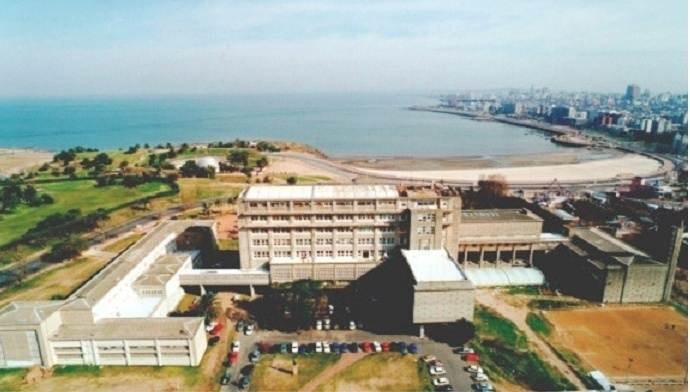
\includegraphics[scale=0.4]{facultad} 
	\end{figure}
}

\frame{\frametitle{Tipos de errores}
\begin{itemize}
\item{\emph{Positivos Verdaderos} (PV) son elementos de la clase buscada que fueron correctamente identificados.}
\item{\emph{Negativos Verdaderos} (NV) son elementos que no pertenecen a la clase buscada que fueron correctamente ignorados y clasificados en una clase diferente.}
\item{\emph{Falsos Positivos} (FP), o errores de Tipo I, son elementos que pertenecen a otra clase y que fueron incorrectamente clasificados en la clase buscada.}
\item{\emph{Falsos Negativos} (FN), o errores de Tipo II, son elementos que pertenecen a clase buscada y que fueron incorrectamente clasificados en otra clase.}
\end{itemize}
}

\frame{\frametitle{Métricas}
\begin{equation}
	\label{eq:precision}
	P = \frac{PV}{PV + FP}
\end{equation}
\begin{equation}
	\label{eq:recall}
	R = \frac{PV}{PV + FN}
\end{equation}
\begin{equation}
	\label{eq:medida-f}
	F_{\alpha} = \frac{P \times R}{(1 - \alpha)P + (\alpha)R}
\end{equation}
\begin{equation}
	\label{eq:medida-f-0-5}
	F_{0.5} = \frac{2 \times P \times R}{P + R}
\end{equation}
}
				
\frame{\frametitle{Ejemplos}									
\begin{itemize}
\small
\item{\emph{Si de él careciéramos, ¿para qu\'e/\texttt{\small SIN\_TILDE} unas tareas que/\texttt{\small SIN\_TILDE} requieren esfuerzo, dedicación, capacidad y que/\texttt{\small SIN\_TILDE} ---además--- no mejoran ninguna economía?}}

\item{\emph{¿No se debate permanentemente ---como/\texttt{\small CON\_TILDE} toda religión y toda de\-men\-cia--- en el conflicto entre lo real y lo ficticio, lo percibido y lo proyectado, lo que/\texttt{\small SIN\_TILDE} constriñe y lo que/\texttt{\small SIN\_TILDE} exalta, los milagros y las bromas pesadas?}}

\item{\emph{-Que/\texttt{\small CON\_TILDE} cómo/\texttt{\small SIN\_TILDE} va a llamarse el chiquillo?}}

%\item{\emph{En esta línea, Alberto Fernández se ha preguntado que/\texttt{\small SIN\_TILDE} ''si esto es lo que/\texttt{\small SIN\_TILDE} ocurrió entonces cuando/\texttt{\small SIN\_TILDE} CiU era influyente en Madrid, ¿qu\'e/\texttt{\small SIN\_TILDE} tiene que/\texttt{\small SIN\_TILDE} pasar ahora con un escenario español totalmente diferente?''}}

%\item{\emph{El dirigente popular ha evitado, no obstante, plantear su oferta de diálogo a CiU en el Parlamento en forma de ultimátum y ha asegurado que/\texttt{\small SIN\_TILDE} el PP ''no se precipitará'' y que/\texttt{\small SIN\_TILDE} espera a ver ''qué/\texttt{\small SIN\_TILDE} ficha mueve'' la coalición que/\texttt{\small SIN\_TILDE} lidera Jordi Pujol.}} 

%\item{\emph{Además, confirmó que/\texttt{\small SIN\_TILDE} la marca de lujo Rolls Royce, adherida igualmente a BMW, permanecerá en el Reino Unido, por su añeja tradición británica y sus dimensiones, mucho menores que/\texttt{\small SIN\_TILDE} Rover, aunque no precisó d\'onde/\texttt{\small SIN\_TILDE} se instalará la nueva planta que/\texttt{\small SIN\_TILDE} la fabricará.}}

\item{\emph{''Un experimento probará la preparación y las capacidades para el contexto militar del futuro, y sirve para que/\texttt{\small SIN\_TILDE} veamos c\'omo/\texttt{\small SIN\_TILDE} cada una de las fuerzas se desempeñará en una guerra''. }}
\end{itemize}													
}																							
% ==============================================================
\end{document}